%%
%% Copyright: Andy GAO (华工自动化)
%%
%%==========================================================
%%          华南理工大学博士学位论文——第二章
%%       Author: Andy GAO        Date: 2022.01.
%%==========================================================
%%

\chapter{实验方法}
\label{cha:Chapter2}


\section{任务A: 视觉检测}
\label{sec:2_Introduction}

引言引言引言引言引言引言引言引言引言引言引言引言引言引言引言引言引言引言引言引言引言引言引言引言引言引言引言引言引言引言引言引言。



\section{任务B: IBVS控制}
\label{sec:2_MechanicalDesign}

机器人的机械结构设计机器人的机械结构设计分别如图{\ref{fig:2_PhysicalWelCH}}与图{\ref{fig:2_VirtualWelCH}}所示。


%
%%%%%%%%%%%%%%%%%%%%%%%%%%%%%%%%%%%%%%%%%%%%%%%%%%%%% Figure
\begin{figure}
  \centering
  \subfloat{
  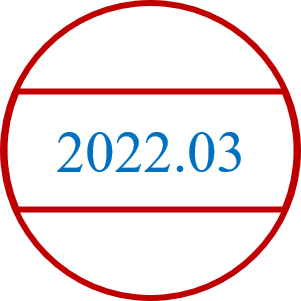
\includegraphics[width=0.45\linewidth,height=0.30\linewidth]{2_Methods/FIGs/tmp} }
  \qquad%\hfill
  \subfloat{
  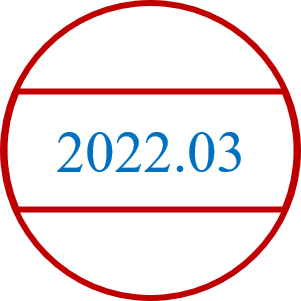
\includegraphics[width=0.45\linewidth,height=0.30\linewidth]{2_Methods/FIGs/tmp} }
  \caption{吸附式攀爬六足机器人WelCH的物理样机模型}
  \label{fig:2_PhysicalWelCH}
\end{figure}
%%%%%%%%%%%%%%%%%%%%%%%%%%%%%%%%%%%%%%%%%%%%%%%%%%%%% End Figure
%


%
%%%%%%%%%%%%%%%%%%%%%%%%%%%%%%%%%%%%%%%%%%%%%%%%%%%%% Figure
\begin{figure}
  \centering
  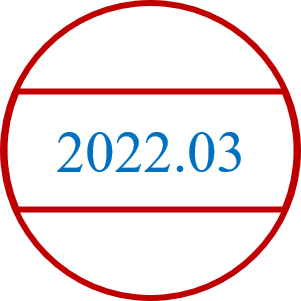
\includegraphics[width=0.5\linewidth]{2_Methods/FIGs/tmp}
  \caption{吸附式攀爬六足机器人WelCH的SolidWorks虚拟原型}
  \label{fig:2_VirtualWelCH}
\end{figure}
%%%%%%%%%%%%%%%%%%%%%%%%%%%%%%%%%%%%%%%%%%%%%%%%%%%%% End Figure
%



\subsection{数学公式数学公式}
\label{sec:2_StructureLayout}

机体与支链结构布局机体与支链结构布局，如图{\ref{fig:2_Body&Limb}\subref{fig:2_BodyOfWelCH}}所示。


%
%%%%%%%%%%%%%%%%%%%%%%%%%%%%%%%%%%%%%%%%%%%%%%%%%%%%% Figure
\begin{figure}[t]
  \centering
  \subfloat[]{ \label{fig:2_BodyOfWelCH}
  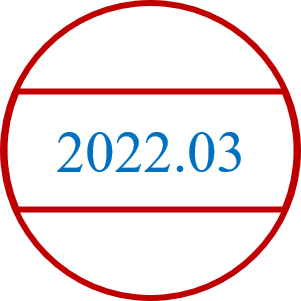
\includegraphics[width=0.35\linewidth,height=0.35\linewidth]{2_Methods/FIGs/tmp}}
  \qquad%\hfill
  \subfloat[]{ \label{fig:2_LimbOfWelCH}
  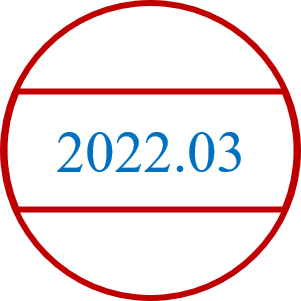
\includegraphics[width=0.35\linewidth,height=0.35\linewidth]{2_Methods/FIGs/tmp}}
  \caption{吸附式攀爬六足机器人WelCH的机体平台与单腿支链的结构布局}
  \label{fig:2_Body&Limb}
\end{figure}
%%%%%%%%%%%%%%%%%%%%%%%%%%%%%%%%%%%%%%%%%%%%%%%%%%%%% End Figure
%


机体与支链结构布局机体与支链结构布局（如图{\ref{fig:2_Body&Limb}\subref{fig:2_LimbOfWelCH}}所示）。
髋关节（记为关节1）的旋转轴线经过连接点$V_{\ell}$且垂直于机体平台平面。。。。。。（对应于关节3相对于关节2存在幅值为$90^{\circ}$ 的初始扭转角），该位形亦称为是六足机器人WelCH的{\it{标称位形}}。
机体与支链结构布局机体与支链结构布局如表{\ref{tab:2_JointRotationRange}}所列。


%
%%%%%%%%%%%%%%%%%%%%%%%%%%%%%%%%%%%%%%%%%%%%%%%%%%%%% Table
\begin{table}[t]
\setstretch{1.5}
\centering
\caption{单腿支链上四个主动关节的有效旋转范围}
\label{tab:2_JointRotationRange}
\begin{tabular}{ccc}
\toprule[1.5pt]
\multirow{2}{*}{旋转副}    &   \multicolumn{2}{c}{关节转动范围}   \\
                               \cline{2-3}
                           &   {角度制（${{}^\circ}$）}     &   {弧度制（${\rm rad}$）} \\
\hline
髋关节（关节1）            &   $[-60, 60]$               &   $[-\frac{\pi}{3}, \frac{\pi}{3}]$ \\
胫关节（关节2）            &   $[-90, 90]$               &   $[-\frac{\pi}{2}, \frac{\pi}{2}]$ \\
膝关节（关节3）            &   $[-45, 80]$               &   $[-\frac{\pi}{4}, \frac{4\pi}{9}]$ \\
踝关节（关节4）            &   $[-90, 90]$               &   $[-\frac{\pi}{2}, \frac{\pi}{2}]$ \\
\bottomrule[1.5pt]
\end{tabular}
\end{table}
%%%%%%%%%%%%%%%%%%%%%%%%%%%%%%%%%%%%%%%%%%%%%%%%%%%%% End Table
%



\subsection{数学公式数学公式数学公式}
\label{sec:2_HardwareDesign}

机器人的硬件系统设计机器人的硬件系统设计如图{\ref{fig:2_HardwareSystem}}所示。


%
%%%%%%%%%%%%%%%%%%%%%%%%%%%%%%%%%%%%%%%%%%%%%%%%%%%%% Figure
\begin{figure}
  \centering
  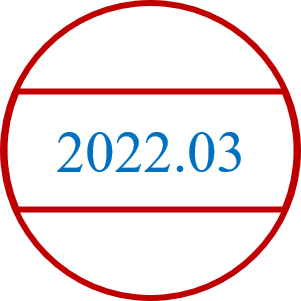
\includegraphics[width=0.9\linewidth]{2_Methods/FIGs/tmp}
  \caption{吸附式攀爬六足机器人WelCH的硬件系统架构图}
  \label{fig:2_HardwareSystem}
\end{figure}
%%%%%%%%%%%%%%%%%%%%%%%%%%%%%%%%%%%%%%%%%%%%%%%%%%%%% End Figure
%


机器人的硬件系统设计机器人的硬件系统设计机器人的硬件系统设计。
该型电机兼具转矩特性良好、效率较高、载荷较强、体量轻小等优点，其部分参数配置如表{\ref{tab:2_ServoMotorConfiguration}}所列。


%
%%%%%%%%%%%%%%%%%%%%%%%%%%%%%%%%%%%%%%%%%%%%%%%%%%%%% Table
\begin{table}
\setstretch{1.5}
\centering
\caption{DCX22L型有刷直流电机的参数配置表}
\label{tab:2_ServoMotorConfiguration}
\begin{tabular}{*{2}{c}@{\hspace{2.5em}}*{2}{c}}
\toprule[1.5pt]
条目                        &       数值            &       条目                            &       数值 \\
\hline
标称电压                    &       48 V            &       空载转速                        &       10100 rpm \\
空载电流                    &       16.2 mA         &       标称转速                        &       9020 rmp \\
标称转矩（最大连续转矩）    &       30.3 mNm        &       标称电流（最大连续电流）        &       0.687 A \\
失速转矩                    &       294 mNm         &       失速电流                        &       6.5 A \\
最大效率                    &       89.9{\%}        &       最大输出功率                    &       45.8 W \\
最大允许转速                &       18000 rpm       &       最大轴向载荷                    &       2.5 N \\
最大径向载荷                &       16 N            &       质量                            &       100 g \\
\bottomrule[1.5pt]
\end{tabular}
\end{table}
%%%%%%%%%%%%%%%%%%%%%%%%%%%%%%%%%%%%%%%%%%%%%%%%%%%%% End Table
%


机器人的硬件系统设计机器人的硬件系统设计。



\section{本章小结}
\label{sec:2_Conclusion}

本章小结本章小结本章小结本章小结本章小结本章小结本章小结本章小结本章小结本章小结本章小结本章小结。


%%
%% Copyright: Andy GAO (华工自动化)
%%
%%==========================================================
%%          华南理工大学博士学位论文——第二章
%%       Author: Andy GAO        Date: 2022.01.
%%==========================================================
%%